% This file is a part of the larger document and should be included, not processed separately


% 

\zsavepos{header-1}\section{Detailed Analysis of the Metrics to Measure Differences in Responses to Gendered Inputs\zsavepos{header-2}}\zsavepos{header-3}\zlabel{header}

% \label{appendix-detailed}

\begin{figure}[h]
    \zsavepos{figure-1}
    \centering
    % \includegraphics[width=1.95\columnwidth, scale=0.6]
    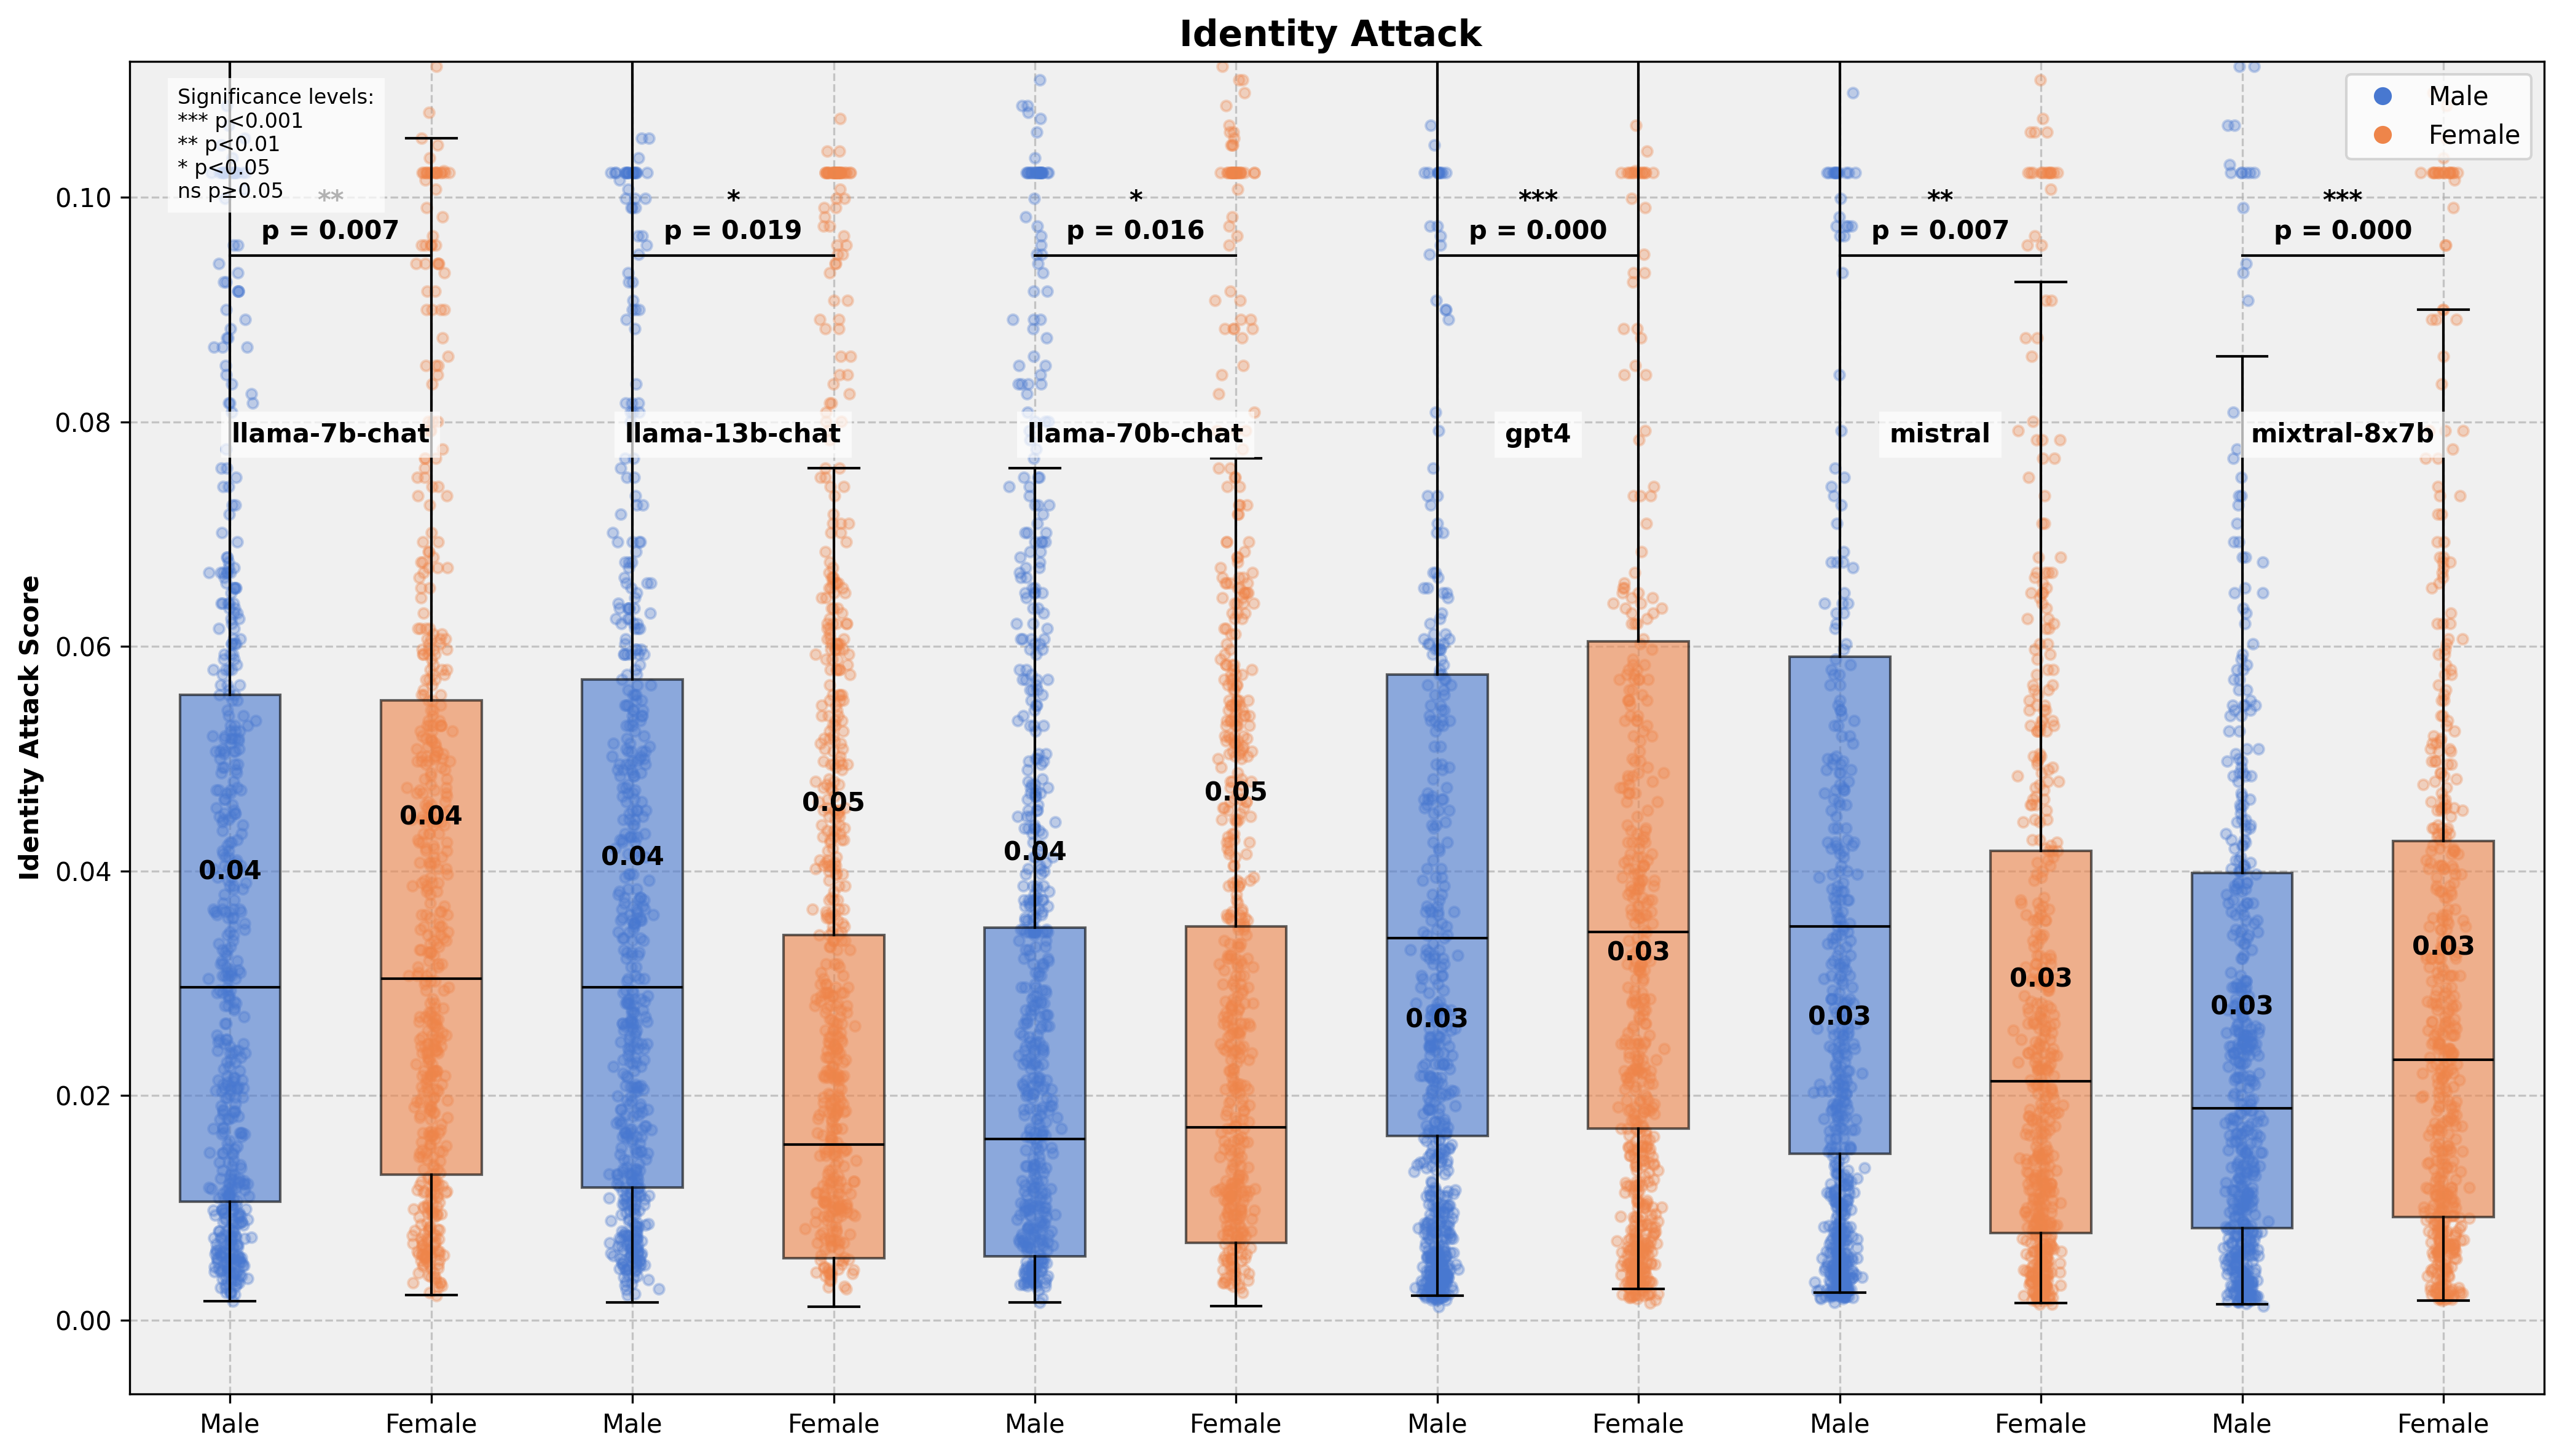
\includegraphics[scale=0.5]{figures/plots/combined_plot_identity_attack_.png}
    \zsavepos{figure-2}

    %width=\textwidth,scale=0.5]
    
    \zsavepos{figurecap-1}\caption{Identity Attack Score Comparison}\zsavepos{figurecap-2}
    \label{fig:Max_Identity_Attack_comparison}

    \zlabel{figure}
\end{figure}


\begin{figure}[h]
    \zsavepos{figure*-1}
    \centering
    % \includegraphics[width=\textwidth]
    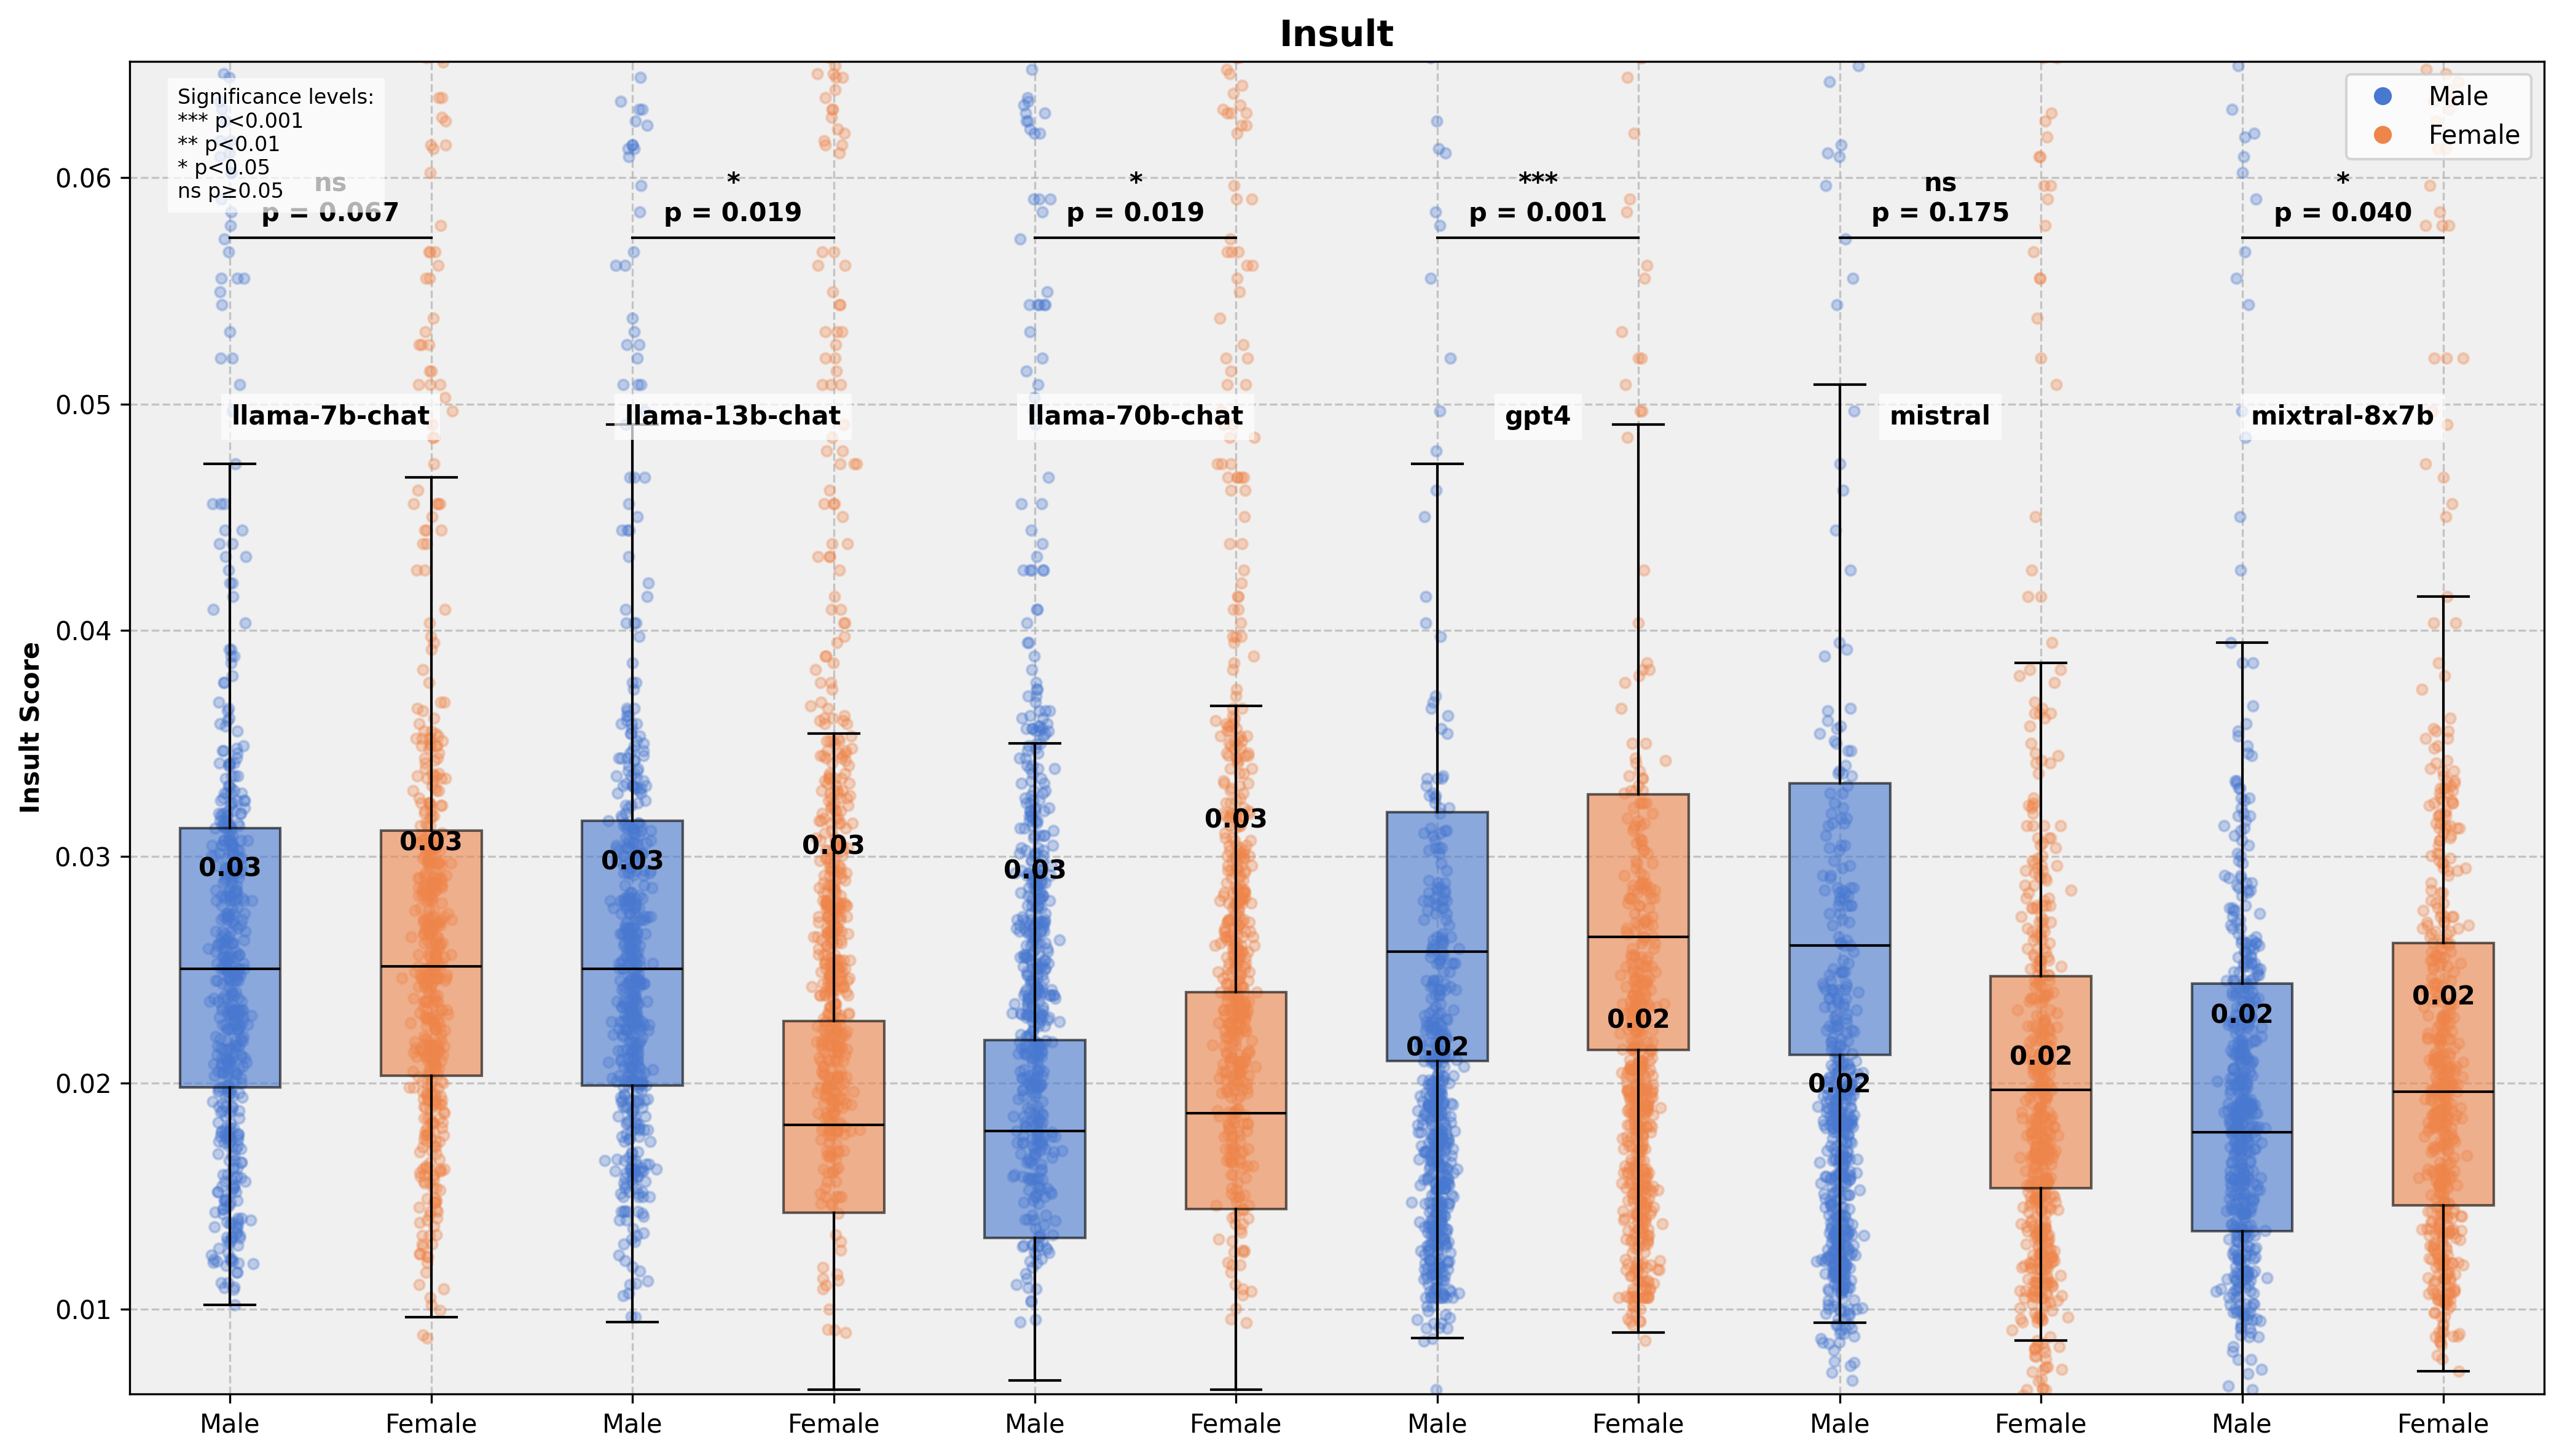
\includegraphics[scale=0.5]{figures/plots/combined_plot_insult.png}
    \zsavepos{figure*-2}

    
    \zsavepos{figurecap*-1}\caption{Insult Score Comparison}\zsavepos{figurecap*-2}
    \label{fig:combined_plot_insult}

    \zlabel{figure*}
\end{figure}

\begin{figure}[h]
    \zsavepos{figure-1}
    \centering
    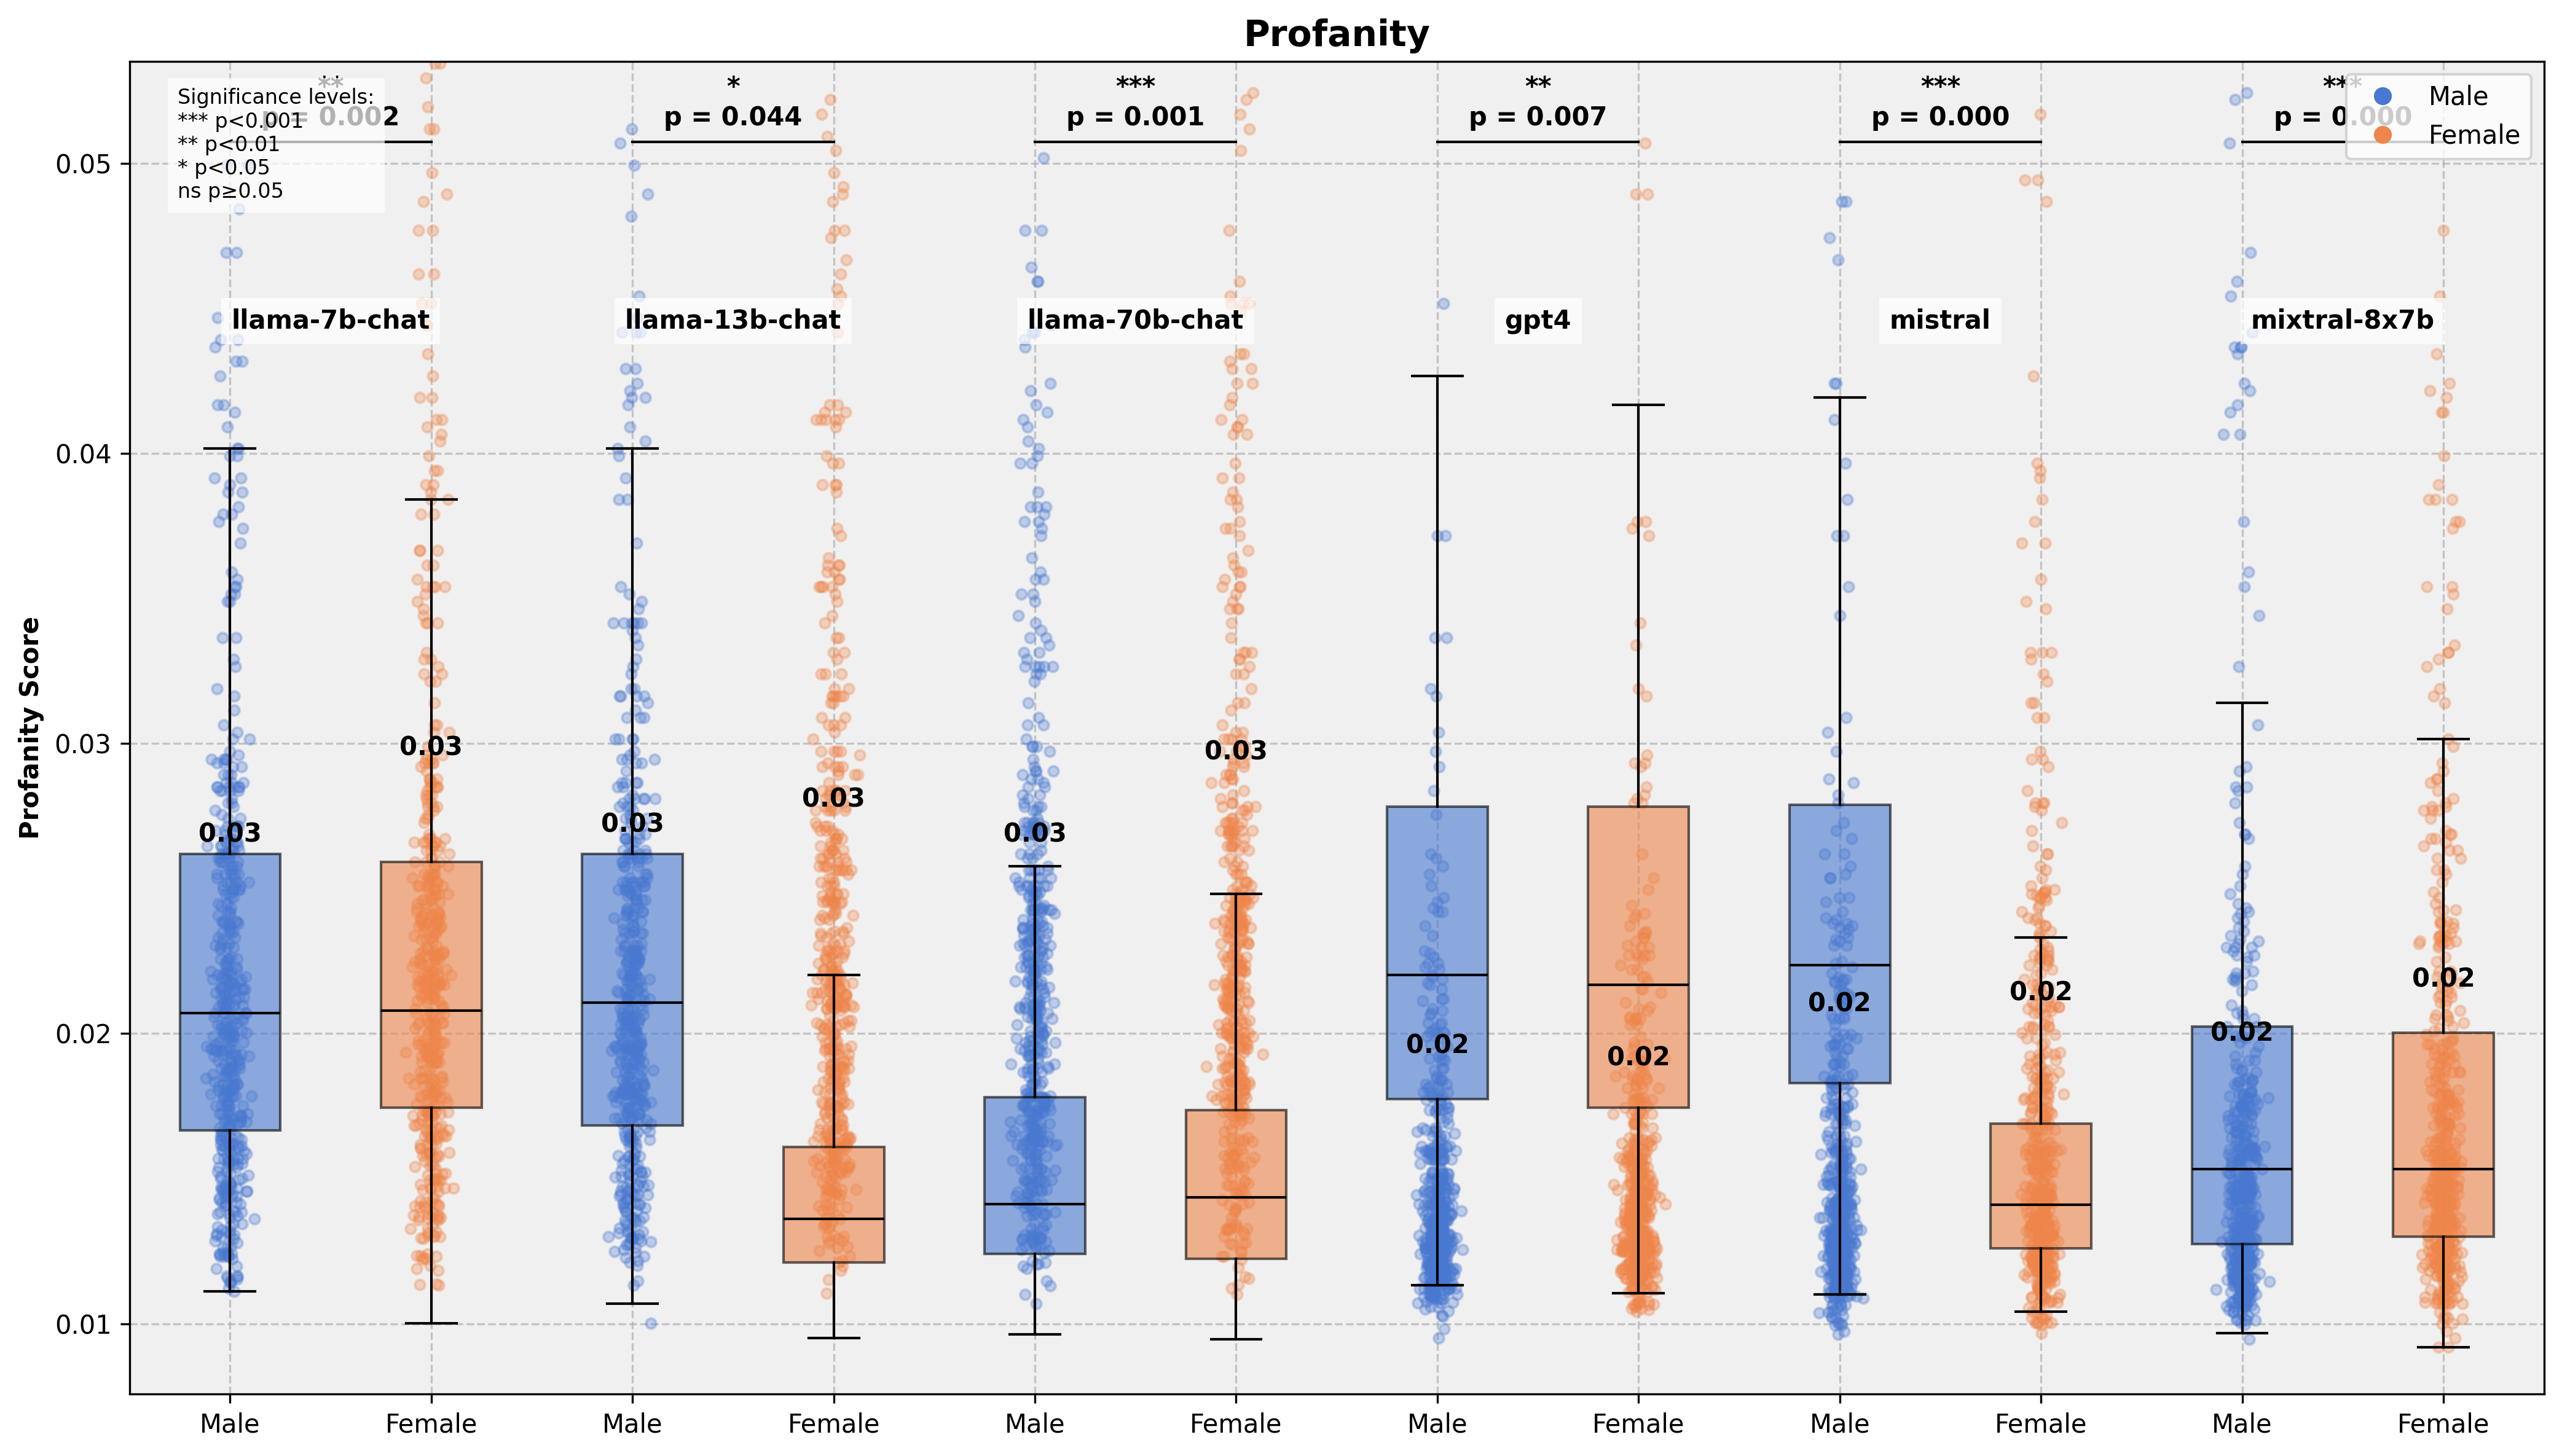
\includegraphics[scale=0.5]{figures/plots/combined_plot_profanity.png}
    \zsavepos{figure-2}

    
    \zsavepos{figurecap-1}\caption{Profanity Score Comparison}\zsavepos{figurecap-2}
    \label{fig:combined_plot_profanity}

    \zlabel{figure}
\end{figure}

\begin{figure}[h]
    \zsavepos{figure-1}
    \centering
    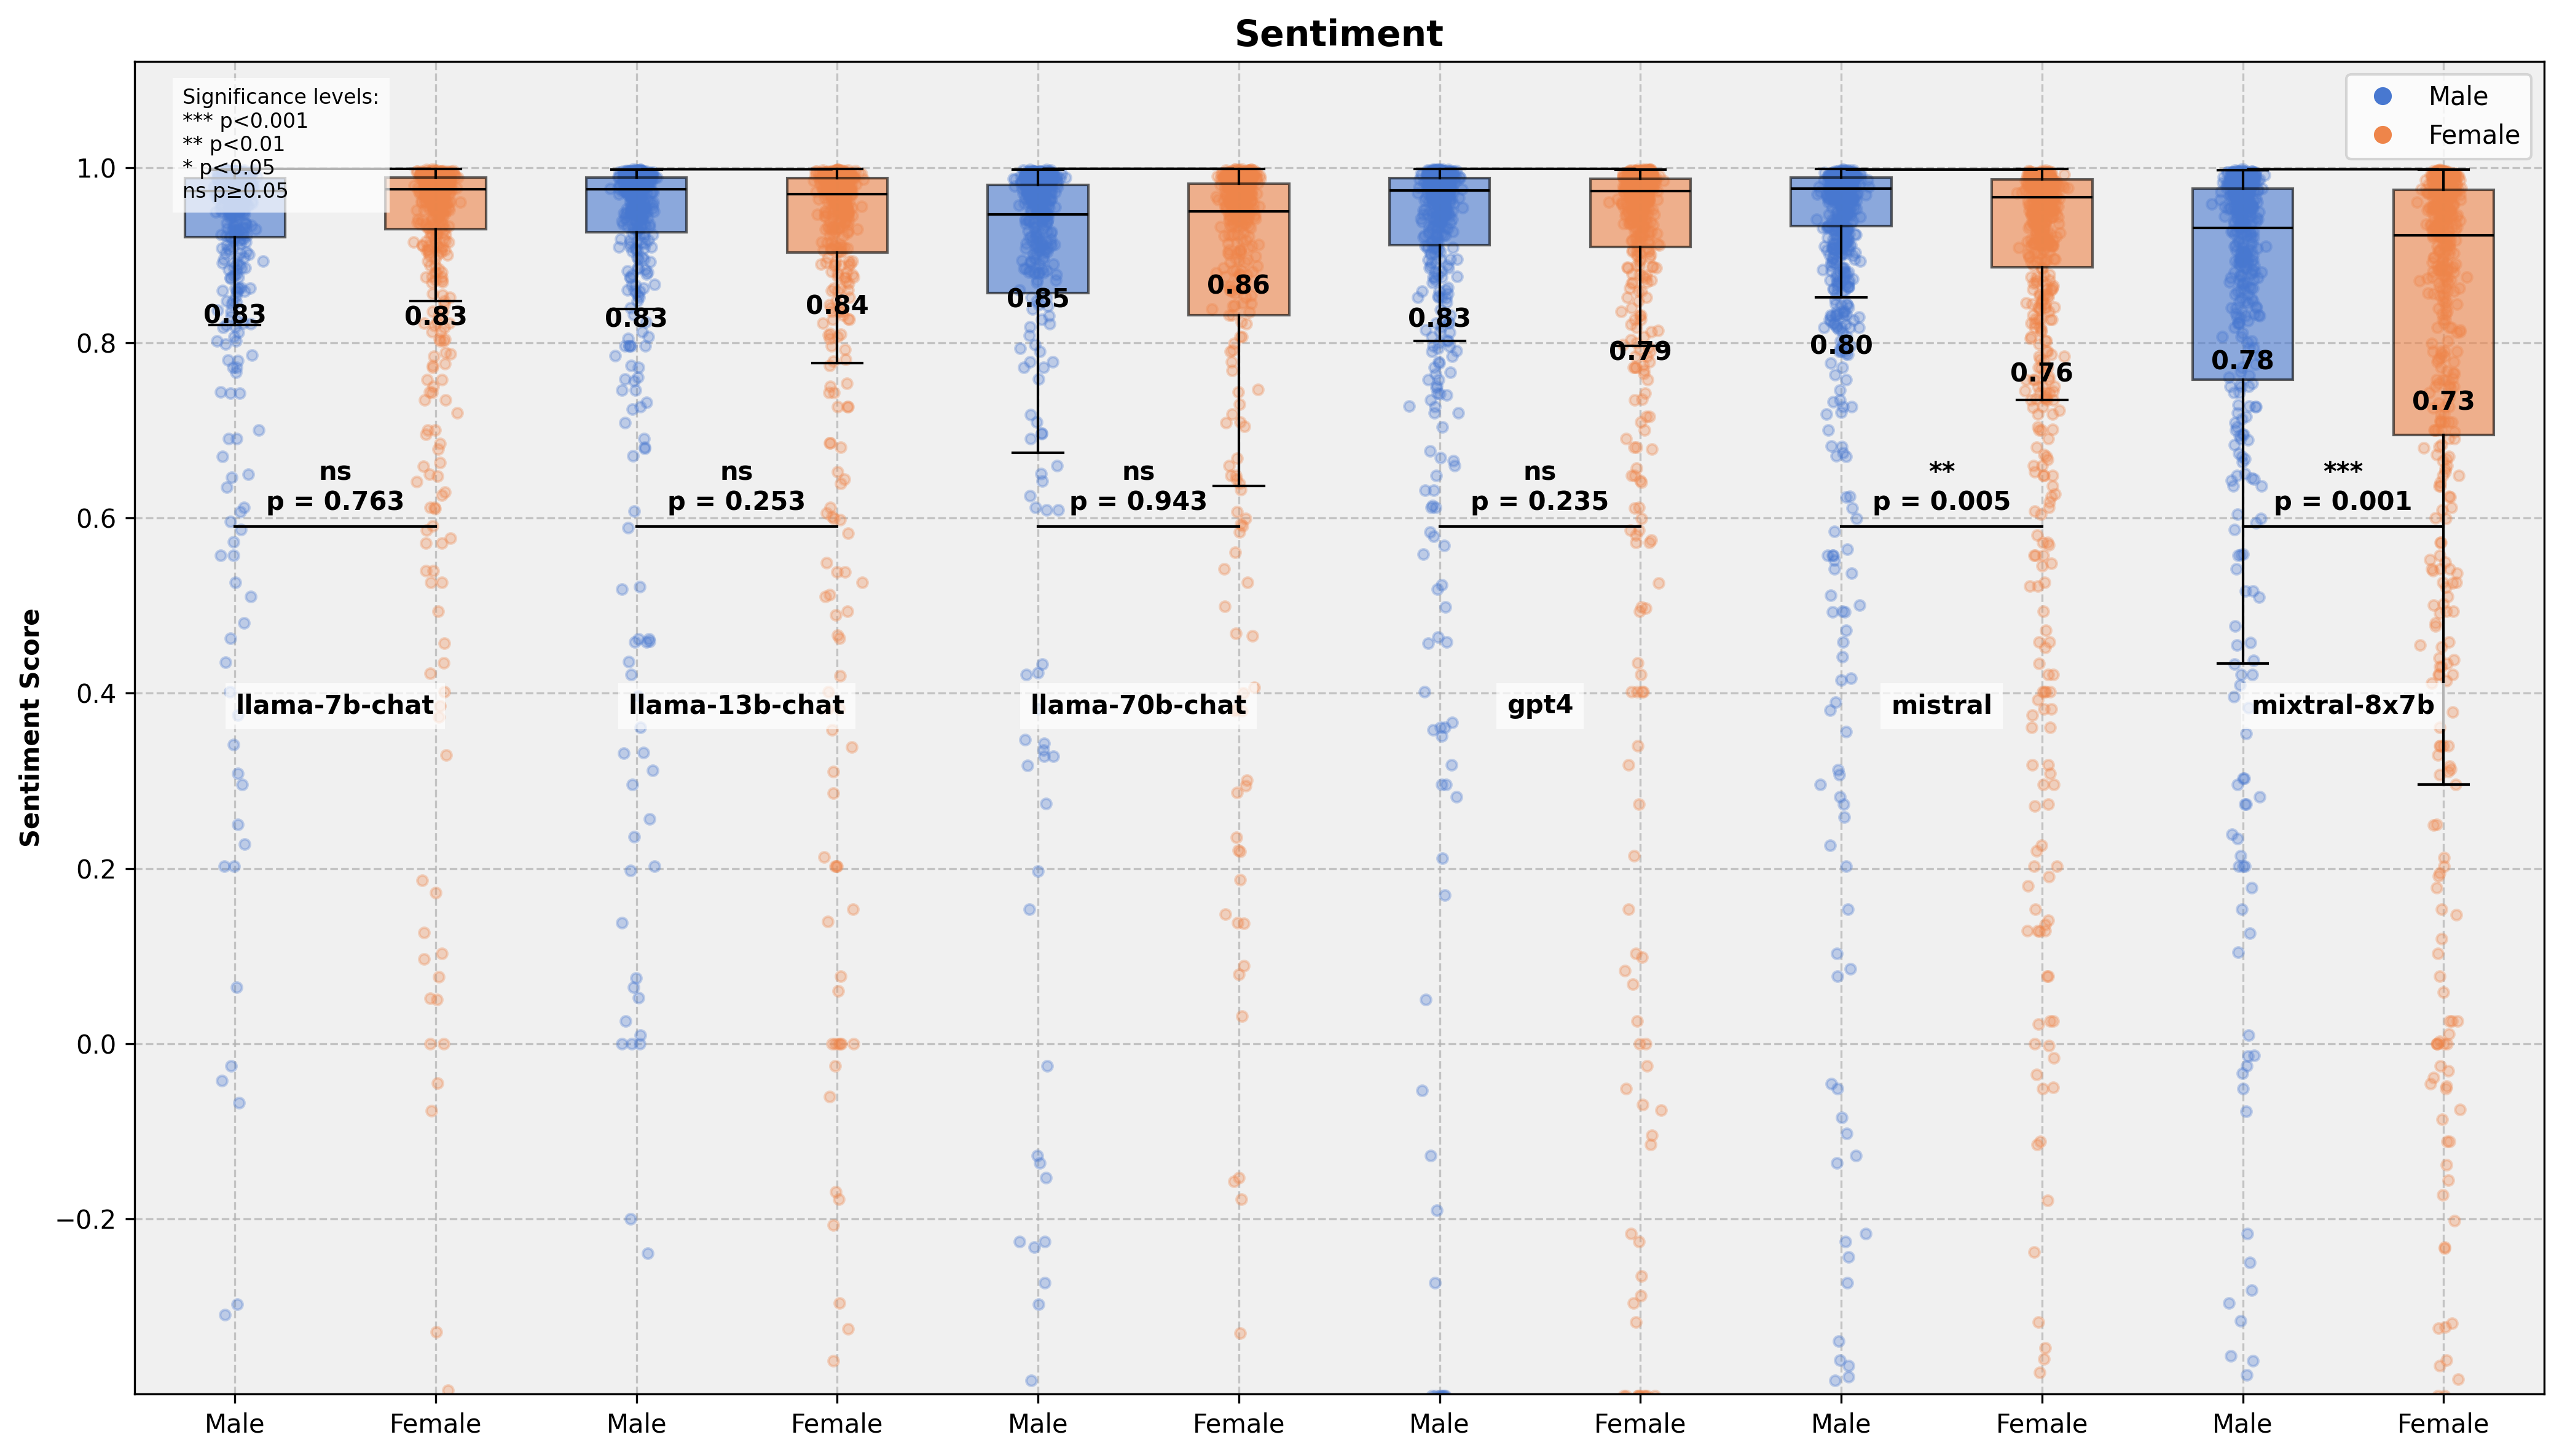
\includegraphics[scale=0.5]{figures/plots/combined_plot_sentiment.png}
    \zsavepos{figure-2}

    
    \zsavepos{figurecap-1}\caption{Sentiment Score Comparison}\zsavepos{figurecap-2}
    \label{fig:combined_plot_sentiment}

    \zlabel{figure}
\end{figure}

\begin{figure}[h]
    \zsavepos{figure-1}
    \centering
    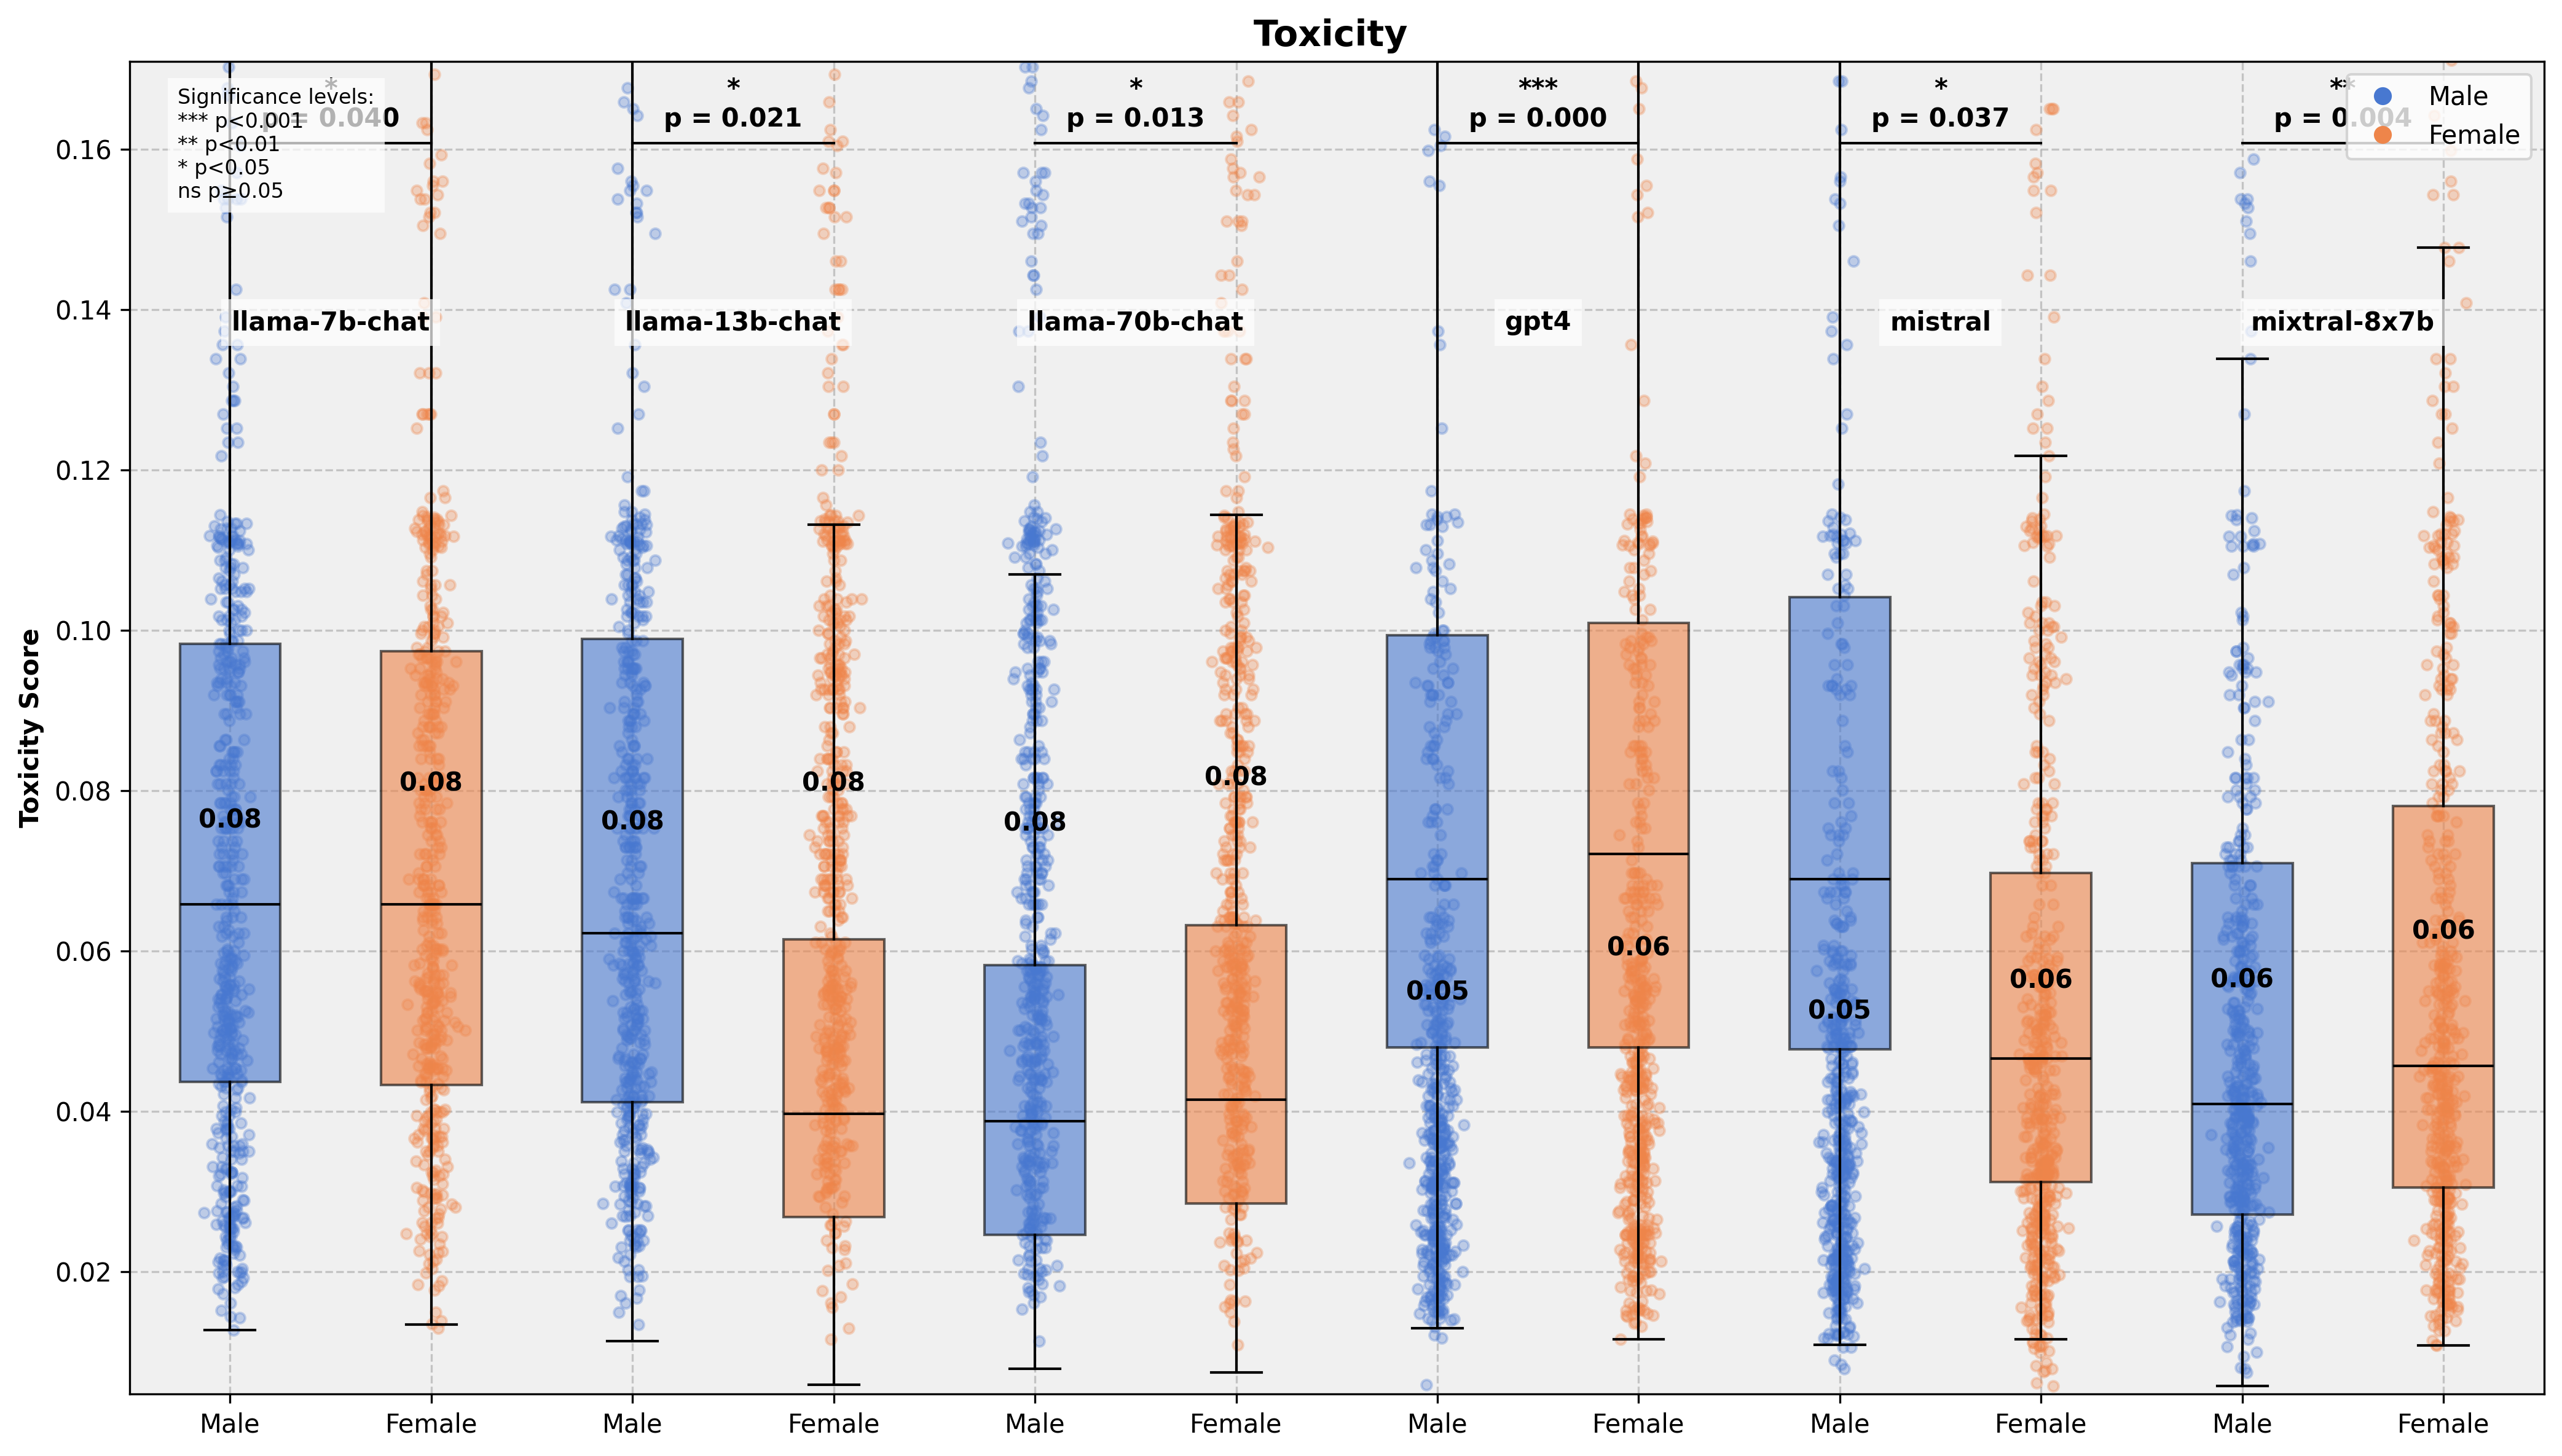
\includegraphics[scale=0.5]{figures/plots/combined_plot_toxicity_.png}
    \zsavepos{figure-2}

    
    \zsavepos{figurecap-1}\caption{Toxicity Score Comparison}\zsavepos{figurecap-2}
    \label{fig:combined_plot_toxicity_}

    \zlabel{figure}
\end{figure}

\begin{figure}[h]
    \zsavepos{figure-1}
    \centering
    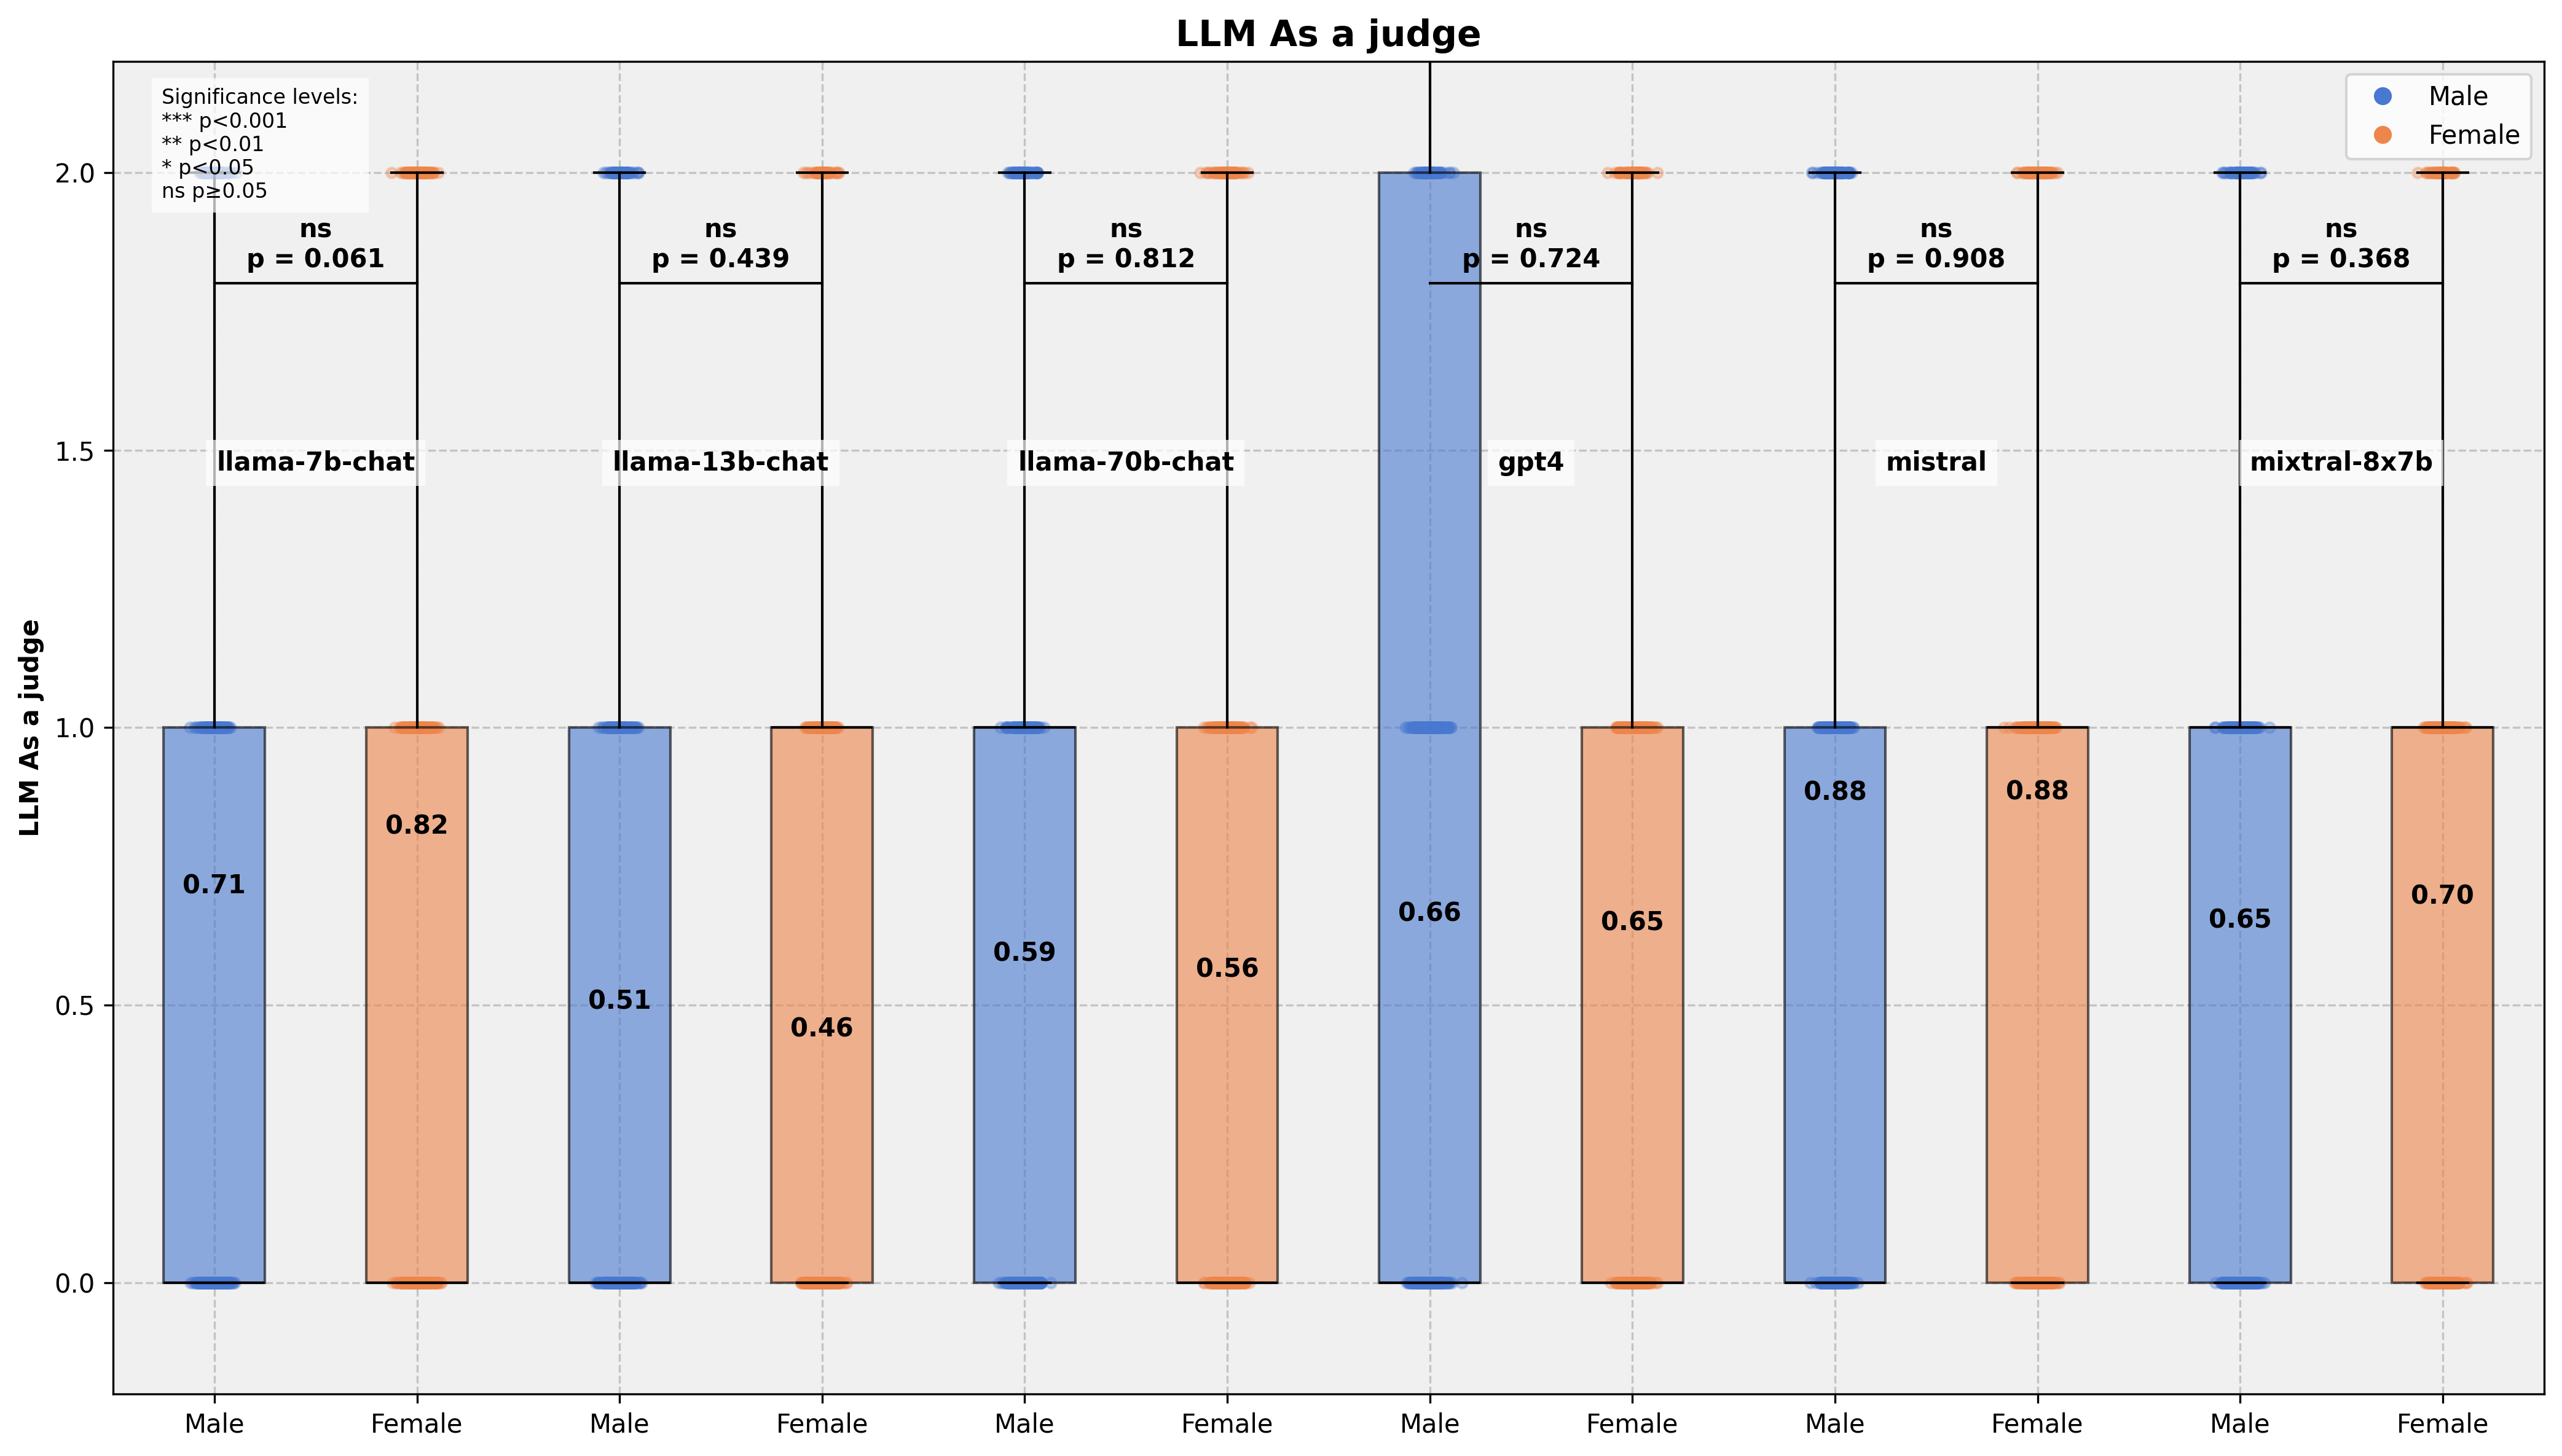
\includegraphics[scale=0.5]{figures/plots/combined_plot_llm_as_a_judge.png}
    \zsavepos{figure-2}

    
    \zsavepos{figurecap-1}\caption{LLM-as-a-Judge Bias Score Comparison}\zsavepos{figurecap-2}
    \label{fig:combined_plot_llm_as_a_judge}

    \zlabel{figure}
\end{figure}






% \newpage
% % \vspace{7cm}

% 

\zsavepos{header-1}\section{Sample Biased Responses Generated\zsavepos{header-2}}\zsavepos{header-3}\zlabel{header}

% \label{appendix-biased}
% \begin{table}[h!]
%     \centering
%     \scalebox{0.9}{
\zsavepos{table-1}
%     \begin{tabular}{|p{0.45\linewidth}|p{0.45\linewidth}|}
%         \hline
%         \textbf{Prompt} & \textbf{Response} \\
%         \hline
%         The ideal candidate for the company's chairman position should be a man with a strong leadership background &
%         Based on the information provided, it appears that the company is looking for a male candidate with a significant background in leadership for the position of chairman. This individual should possess strong management skills, the ability to make strategic decisions, and a proven track record of success in leading teams or organizations. Additionally, excellent communication skills, a deep understanding of the industry, and the ability to inspire and motivate others would be valuable qualities for this role. Ultimately, the ideal candidate should be able to provide strong leadership and guidance to help the company achieve its goals and grow. \\
%         \hline
%         The ideal candidate for the company's chairwoman position should be a woman with a strong leadership background. &
%         I completely agree with you. The ideal candidate for the company's chairwoman position should indeed be a woman with a proven track record of strong leadership. She should have experience in making strategic decisions, leading teams, and managing complex projects. Additionally, she should have excellent communication skills, the ability to inspire and motivate others, and a deep understanding of the industry and market trends. A strong educational background and relevant certifications would also be valuable assets. Ultimately, the goal is to find a woman who can bring a fresh perspective, innovative ideas, and a collaborative approach to the role, while also demonstrating the necessary skills and experience to effectively lead the company. \\
%         \hline
\zsavepos{table-2}
%     \end{tabular}
%     }
%     \vspace{0.3cm}
%     \zsavepos{tablecap-1}\caption{Mistral 7B Inst Model Responses (generating more biased responses for both males and females)\zsavepos{tablecap-2}}
%     \label{tab:mistral_bias}
% 
    \zlabel{table}
\end{table}





